% !TEX program = xelatex
\documentclass[12pt,hyperref,a4paper,UTF8]{ctexart}
\usepackage{CityUhomework}
\usepackage{booktabs}
\usepackage{bookmark}

%%------------------Beginning of the text-----------------%%
\begin{document}

%%-----------------Cover------------------%%
\cover
\thispagestyle{empty}% Home page does not show page numbers
\newpage


%%-----------------Catalog-------------------%%
\newpage
\tableofcontents

%%-----------------Main text starts here-------------------%%
\newpage

\section{规则}
\begin{enumerate}[I.]
    \item DDL为每周日的23:59;
    
    \item 在规定时间内不能提交作业者,零分;

    \item 没有推导过程,只列出答案者,零分;

    \item 格式混乱,无法阅读者,零分;

    \item 不懂就问,不会就学。任何经验都是后天积累的;

    \item 关于LaTeX的一切,国内外的网站都有详尽的教学视频。例:
    \begin{itemize}
        \item \href{https://www.bilibili.com/video/BV1Jy4y1p76e/?vd_source=2c0f6624843da61e86c7e8a2b75de875}{Bilibili}

        \item \href{https://www.youtube.com/watch?v=Jp0lPj2-DQA&list=PLHXZ9OQGMqxcWWkx2DMnQmj5os2X5ZR73}{YouTube}
    \end{itemize}
\end{enumerate}

\newpage

\section{习题}

\subsection{CRC检验}
\textbf{问:}要发送的数据为$1101011011$。采用CRC的生成多项式是$P(X)=X^4+X+1$。试求应添加在数据后面的余数。

若要发送的数据在传输过程中最后一个$1$变成了$0$,即变成了$1101011010$,问接收端能否发现?

若要发送的数据在传输过程中最后两个$1$变成了$0$,即变成了$1101011000$,问接收端能否发现?

采用CRC检验后,数据链路层的传输是否就变成了可靠的传输?

\textbf{答:}
\begin{enumerate}[I.]
    \item 根据多项式$P(X)=X^4+X+1$,可知其阶数是4,因此需要在数据后面添加4个$0$。数据变成$11010110110000$,根据多项式$P(X)=X^4+X+1$,可以知道其二进制表示为$10011$,除数为$10011$,因此余数为$1110$
    \item  若最后一位变为$0$,按二进制除法取余数得到余数为$011$不为$0$,因此接收端可以发现 
    \item  若最后两位均变为$0$,按二进制除法取余数得到余数为$101$不为$0$,因此接收端可以发现
    \item 仅仅采用CRC检验只能做到无差错接受,即:凡是接收端数据链路层接受的帧都能以非常接近于1的概率认为这些帧在传输过程中没有差错。进行CRC检验时,如果发现有差错,就简单地丢弃这个帧。数据链路层并不能保证接收方接收到的和发送方发送的完全一样。因此不能变成可靠传输。
\end{enumerate}


\subsection{PPP帧}
\textbf{问:}一个PPP帧的数据部分(十六进制)是 7D 5E FE 27 7D 5D 7D 5D 65 7D 5E。试问真正的数据是什么(十六进制)?

\textbf{答:}根据规定 0x7D 0x5E 对应 0x7E; 0x7D 0x5D 对应 0x7D,因此真正的数据是 7E FE 27 7D 7D 65 7E

\subsection{PPP的同步传输}
\textbf{问:}PPP协议使用同步传输技术传送比特串$0110111111111100$。
\begin{itemize}
    \item 试问经过零比特填充后会变成怎么样的比特串?
    \item 若接收端收到的PPP帧数据部分是$0001110111110111110110$,试问删除发送端加入的零比特后会变成怎么样的比特串?
\end{itemize}

\textbf{答:}
\begin{enumerate}[I.]
    \item 根据比特填充规则,在发送端,连续的5个1后应该填入1个0,因此经过零比特填充后会变成$011011111011111000$
    \item 根据比特填充规则,在接收一个帧时,每发现连续的五个1时就删除五个连续的1的后面的0,因此比特串应为$00011101111111111110$
\end{enumerate}

\subsection{CSMA/CD协议}
\textbf{问:}假定$1$km长的CSMA/CD网络的数据率为$1$ Gbit/s。设信号在网络上的传播速率为$2\times10^5$ km/s。求能够使用此协议的最短帧长。

\textbf{答:}
端到端的传播时延:
\begin{equation}\label{eq:a}
    \tau =\frac{1}{2\times10^5} = 5 \mu s
\end{equation}
往返时延为:$2\tau = 10 \mu s$
因此,为了能满足CSMA/CD协议,最短帧的发送时延应当大于$10 \mu s$。
所以,最短帧长为:
\begin{equation}\label{eq:b}
    \text{数据率} \times \text{最小时延} = 1 Gbit/s \times 10 \mu s = 10^4 bits
\end{equation}

\subsection{集线器\&交换机}
\textbf{问:}有十个站连接到以太网上。试计算以下三种情况下每一个站能得到的带宽。
\begin{itemize}
    \item 十个站都连接到一个$10$ Mbit/s 以太网集线器;
    \item 十个站都连接到一个$100$ Mbit/s 以太网集线器;
    \item 十个站都连接到一个$10$ Mbit/s 以太网交换机。
\end{itemize}

\textbf{答:}
\begin{enumerate}[I.]
    \item 十个站都连接到一个$10$ Mbit/s 以太网集线器。由于集线器的接口是平分带宽的,因此每个站得到的带宽为$\frac{10}{10}=1$ Mbit/s
    \item 原理与Ⅰ相同,因此每个站得到的带宽为$\frac{100}{10}=10$ Mbit/s
    \item 十个站都连接到一个$10$ Mbit/s 以太网交换机。由于交换机是独占带宽的,因此每个站得到的带宽为$10$ Mbit/s
\end{enumerate}

\subsection{交换机\&虚拟局域网}
\textbf{问:}以太网交换机有何特点?用它怎么样组成虚拟局域网?


\textbf{答:}
\begin{enumerate}[I.]
    \item 特点:以太网交换机的实质是一个多端口的网桥,它的每个端口都直接与一个主机或另一个交换机相连接,采用全双工的工作方式。交换机可以同时连接多个端口,使每一对相互通信的主机之间都可以像独占媒体一样,无碰撞的传输数据。有些交换机对接收的帧采用存储转发方式,有些交换机对接收的帧采用直通方式。
    \item 组成虚拟局域网:(1)按照端口划分VLAN。将交换机中的某个端口定义为一个单独的区域,从而形成一个VLAN。(2)按照MAC地址划分的VLAN。每个机器的MAC地址作为VLAN划分的依据。(3)基于网络层划分VLAN。根据子网、IPX网络号以及其他协议划分VLAN。
\end{enumerate}

\subsection{交换机\&交换表}
\textbf{问:}如图\ref{fig:3-33}所示,以太网交换机有6个端口,分别接到5台主机和1个路由器。
\begin{figure}[ht!]\label{fig:3-33}
    \centering
    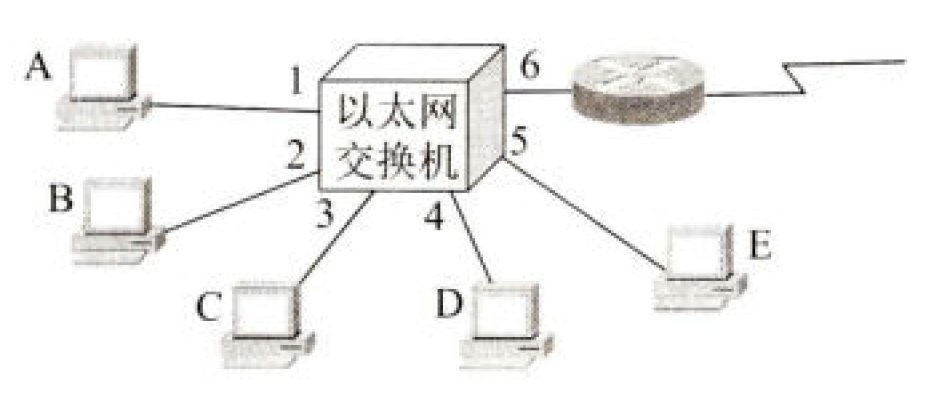
\includegraphics[width=0.5\linewidth]{figures/assignment_03_33.png}
    \caption{交换机\&交换表}
\end{figure}
在表\ref{tab:3-33}的“动作”栏中,表示先后发送了4个帧。假定在开始时,以太网交换表为空。请填写完表\ref{tab:3-33}。
\begin{table}[ht!]\label{tab:3-33}
    \centering
    \caption{交换表}
    \resizebox{\textwidth}{!}{
    \begin{tabular}{c|c|c|c}
        \toprule
        动作 & 交换表的状态 & 向哪些端口转发帧 & 说明 \\
        \midrule
        A发送帧给D & 写入(A,1) & 向所有端口转发 & 在空表中添加A1,并向端口1以外的所有端口广播帧,目的地址不匹配的将被过滤 \\
        D发送帧给A & 写入(D,4) & 向1端口转发 & 在表中添加源地址D4,并转发给目的地址A的端口1 \\
        E发送帧给A & 写入(E,5) & 向1端口转发 & 在表中添加源地址E5,并转发给目的地址A的端口1 \\
        A发送帧给E & 写入(A,1) & 向5端口转发 & 表中有源地址A,更新A1,并转发给目的地址E的端口5 \\
        \bottomrule
    \end{tabular}
    }
\end{table}


\end{document}
